\documentclass[10pt]{llncs}
\usepackage{graphicx}
\usepackage{times}
\usepackage{amsmath}
\usepackage{amssymb}
\usepackage[hyphens]{url}
\usepackage{xspace}
\usepackage{microtype}
% \usepackage[showframe]{geometry} % Solo para verificación, quitar en versión final
\usepackage{calc}
\usepackage{xcolor} % Para colores
\usepackage[colorlinks=true]{hyperref} % Enlaces clickeables
\hypersetup{
    linkcolor=blue,
    citecolor=blue,
    filecolor=blue,
    urlcolor=blue
}

% Personalización de referencias cruzadas
\usepackage{cleveref} % Paquete esencial

\crefname{figure}{Fig.}{Figs.} % Para figuras
\crefname{table}{Tab.}{Tabs.} % Para tablas
\crefname{equation}{Ec.}{Ecs.} % Para ecuaciones
\crefname{section}{Sec.}{Secs.} % Para secciones
% Configuración específica para tablas
\crefname{table}{Tab.}{Tabs.} % Singular y plural
\Crefname{table}{Tabla}{Tablas} % Para \Cref (inicio de oración)

% Configuración para LNCS (opcional)
\newcommand{\figref}[1]{\hyperref[#1]{Fig.~\ref*{#1}}}
\newcommand{\tabref}[1]{\hyperref[#1]{Tab.~\ref*{#1}}}
\newcommand{\secref}[1]{\hyperref[#1]{Sec.~\ref*{#1}}}

% Centrado completo del contenido (122mm x 193mm)
\setlength{\textwidth}{122mm}
\setlength{\textheight}{193mm}
\setlength{\oddsidemargin}{(\paperwidth - \textwidth)/2 - 1in}
\setlength{\evensidemargin}{(\paperwidth - \textwidth)/2 - 1in}
\setlength{\topmargin}{(\paperheight - \textheight - \headheight - \headsep - \footskip)/2 - 1in}

% Configuración adicional para cumplir requisitos
\setlength{\parindent}{0pt} % Sin sangría inicial
\frenchspacing % Espaciado adecuado después de puntos
\sloppy % Mejor manejo de división de palabras

% Abstract con márgenes de 1.0cm
\renewenvironment{abstract}{%
  \small
  \begin{list}{}{%
    \setlength{\leftmargin}{1cm}%
    \setlength{\rightmargin}{1cm}%
  }
  \item\relax\ignorespaces}
  {\end{list}\vspace{2\baselineskip}}

% Palabras clave
\newcommand{\keywords}[1]{\par\noindent\textbf{Keywords:} #1}

% Entorno para Remarks
% \newenvironment{remark}
%   {\par\noindent\textit{Remark.} \ignorespaces}
%   {\par}

% Configuración de figuras
\setlength{\abovecaptionskip}{8mm} % Espacio texto-figura
\setlength{\belowcaptionskip}{6mm} % Espacio figura-leyenda
\setlength{\textfloatsep}{10pt} % Espacio entre flotantes

\begin{document}

\title{GPTur}
\titlerunning{Título abreviado} % Sugerencia para running head

\author{Claudia Hernández Pérez \and Joel Aparicio Tamayo \and Kendry Javier Del Pino Barbosa}
\authorrunning{Autor1 et al.} % Apellidos para running head

\institute{
Facultad de Matemática y Computación, La Habana, Cuba
}

\maketitle

\begin{abstract} \textbf{Resumen.}
GPTur es un sistema diseñado con una arquitectura de Generación Aumentada por Recuperación (RAG) con agentes especializados para cada funcionalidad y una base de datos 
vectorial para la recuperación de la información. Posee, además, varios agentes encargados de tópicos específicos como gastronomía, 
vida nocturna, alojamiento y lugares históricos, que comparten datos en una pizarra central. Estos 
agentes están dirigidos por un guía y un planificador. El primero se encarga de responder consultas mientras el segundo utiliza algoritmos para planear 
itinerarios ajustados a presupuestos. Este agente resuelve un problema de satisfacción de restricciones utilizando la técnica de precocido simulado. También, el programa 
preprocesa la consulta para obtener ciertas entidades, palabras claves y sentimientos que puedan influir en los resultados esperados. Todo eso, permite conformar una respuesta acertada, 
acorde a las necesidades del usuario, validadas experimentalmente.
\par
\vspace{2\baselineskip}
\textbf{Palabras clave:} RAG, agente, problema de satisfacción de restricciones, precocido simulado
\end{abstract}

\section{Introducción}\label{sec:intro}
La industria turística enfrenta desafíos únicos en contextos con limitaciones en la infraestructura digital y 
actualización constante de servicios. Cuba, como destino turístico emblemático, requiere soluciones 
innovadoras que superen estas barreras mediante inteligencia artificial. \textit{GPTur}, 
un sistema de agentes inteligentes que funciona como guía turístico virtual, está diseñado específicamente 
para ser una alternativa viable en ese escenario.

La aplicación consiste en un chatbot capaz de responder consultas sobre destinos turísticos cubanos y sus peculiaridades, así como de generar itinerarios para \textit{tours} ajustándose a un presupuesto. 
El sistema está programado en \textit{Python}, aprovechando la comodidad del lenguaje y la diversidad de bibliotecas útiles que ofrece. La interfaz está diseñada con \textit{streamlit} (framework de \textit{Python} para \textit{frontend}), 
pues ofrece un estilo sencillo, moderno y fácil de programar para entornos web. El código fuente de la aplicación se puede encontrar en 
la plataforma GitHub: \href{https://github.com/ClaudiaHdezPerez/GPTur}{\color{blue}https://github.com/ClaudiaHdezPerez/GPTur}.

\section{Detalles de Implementación}\label{sec:implementacion}

En esta sección, se abordarán los distintos temas asociados a la implementación de la solución propuesta, que incluyen la arquitecura RAG y multiagente, funcionamiento del \textit{crawler} automatizado y recopilación del corpus, base de datos vactorial y representación semántica del 
conocimiento mediante \textit{embeddings}, procesamiento de lenguaje natural, algoritmos basados en metaheurísticas, entre otros. 

\vspace{\baselineskip}

\subsection{Arquitectura RAG (\textit{Generación Aumentada por Recuperación})}\label{sec:rag}

Un sistema de Generación Aumentada por Recuperación combina generación de texto con recuperación de información para mejorar la calidad, precisión y actualidad de las respuestas obtenidas de los modelos de lenguaje. 
Está compuesto por una entrada, un recuperador, un generador y una salida. La implementación propuesta es bastante sencilla, ajustada a la definición:
\begin{enumerate}
    \item Entrada: constituida por la consulta del usuario en lenguaje natural.
    \item Recuperador: agente que recibe la consulta y le pide a la base de datos vectorial que recupere la información relacionada.
    \item Generador: agente que utiliza la consulta y la información recuperada para decidir si la respuesta debe ser generada por el guía o el planificador. Para tomar esa decisión le pide a un modelo de lenguaje que detecte la intención del usuario.
    \item Salida: respuesta generada por el agente inteligente encargado de elaborarla.
\end{enumerate}

\vspace{\baselineskip}
\subsection{Arquitectura multiagente}

Un sistema multiagente está constituido por un conjunto de agentes, cada uno con determinadas capacidades y recursos para la solución de problemas inherentemente distribuidos. Los agentes interactúan entre ellos, determinan y coordinan tareas a realizar según sus capacidades y recursos.

GPTur cuenta con dos agentes fundamentales: el guía y el planificador. Existen, además, 
otros especializados en distintos tópicos: gastronomía, vida nocturna, alojamiento y lugares históricos. Todos ellos 

\subsubsection{Información adicional}\label{sec:info}
Encabezados de tercer nivel en 10pt negrita.

\section{Validación y Experimentación}

Esta sección fue un elemento esencial en la etapa de desarrollo y, en muchos casos, influyó en la toma de decisiones. Se realizaron varios experimentos, que incluyen valoraciones de la respuesta del sistema y evaluación de los algoritmos de metaheurísticas.
\vspace{\baselineskip}
\subsection{Respuesta del Sistema}

Durante las distintas etapas de desarrollo, fue importante evaluar el comportamiento de la aplicación. Para estos experimentos se utilizó un modelo de lenguaje para generar 30 preguntas relacionadas con el corpus y obtener las respuestas de GPTur automáticamente. Luego, 
se creó una cosulta para un modelo de lenguaje pidiendo una evaluación entre 0 y 5 puntos de la respuesta del sistema en cuanto a:
\begin{itemize}
    \item  Precisión de la información
    \item Coherencia y relevancia
    \item Cobertura del tema
    \item Calidad de las recomendaciones
    \item Ajuste a la pregunta realizada
\end{itemize}

Después de obtener los resultados de la muestra, se hacía necesario evaluar muestras mucho más grandes, pero eso requería demasiado cómputo, así que como alternativa se utilizó la técnica conocida como \textit{bootstrapping}, pudiendo estudiar muestras de tamaño 300 con 1000 simulaciones. A continuación se muestran los resultados obtenidos 
en las distintas etapas.

\subsubsection{Sistema con Agentes Guía y Planificador Solamente}

La Tabla \tabref{tab:boot_results_1} resume las métricas clave obtenidas:

\begin{table}[h]
\centering
\caption{Resultados del análisis de bootstrapping (IC 95\%)}
\label{tab:boot_results_1}
\begin{tabular}{lccc}
\hline
\textbf{Métrica} & \textbf{Tamaño=30} & \textbf{Tamaño=300}  \\
\hline 
Puntuación Media& 3.7 & 3.7013...  \\
Desviación Estándar & 0.4582... & 0.0261...  \\
\hline
\end{tabular}
\end{table}

\begin{figure}[h]
\centering
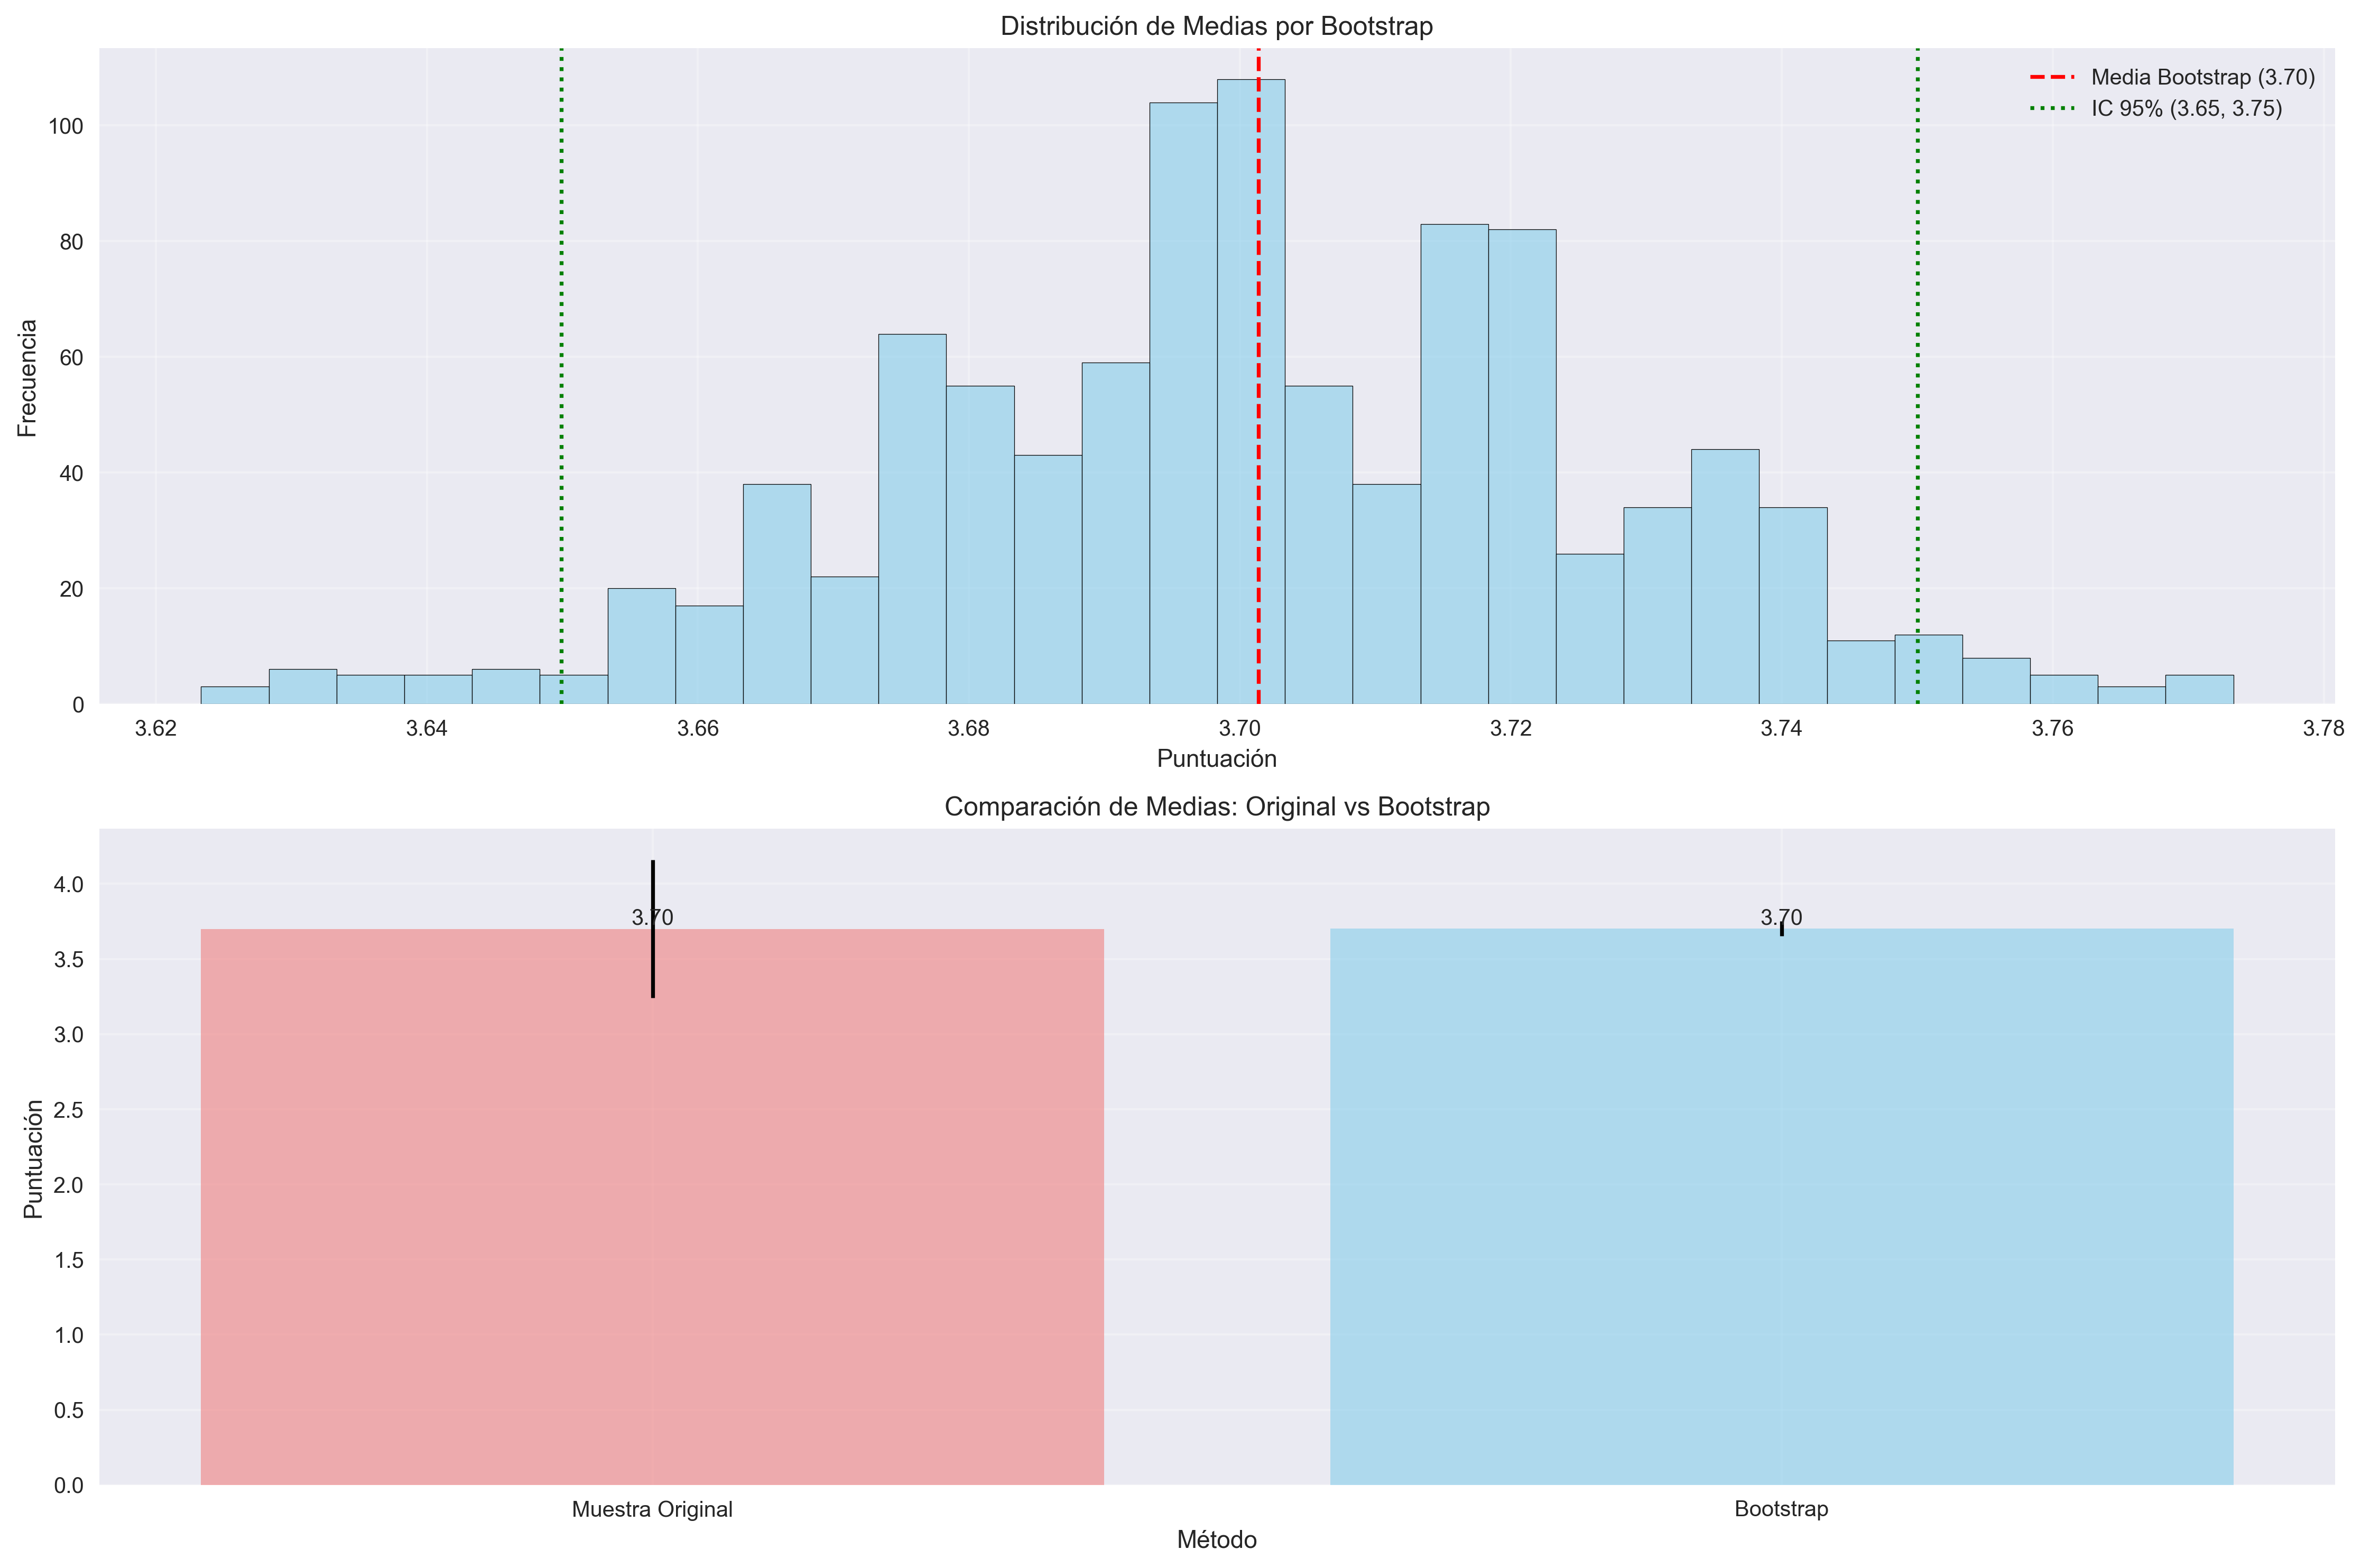
\includegraphics[width=1\textwidth]{../src/experiments/one_only_agent/bootstrap_distribution_20250614-143724.png}
\caption{Distribución bootstrap de la puntuación media ($N=1000$). La línea discontinua roja indica la media bootstrap (3.70)}
\label{fig:boot_dist_1}
\end{figure}

\begin{figure}[h]
\centering
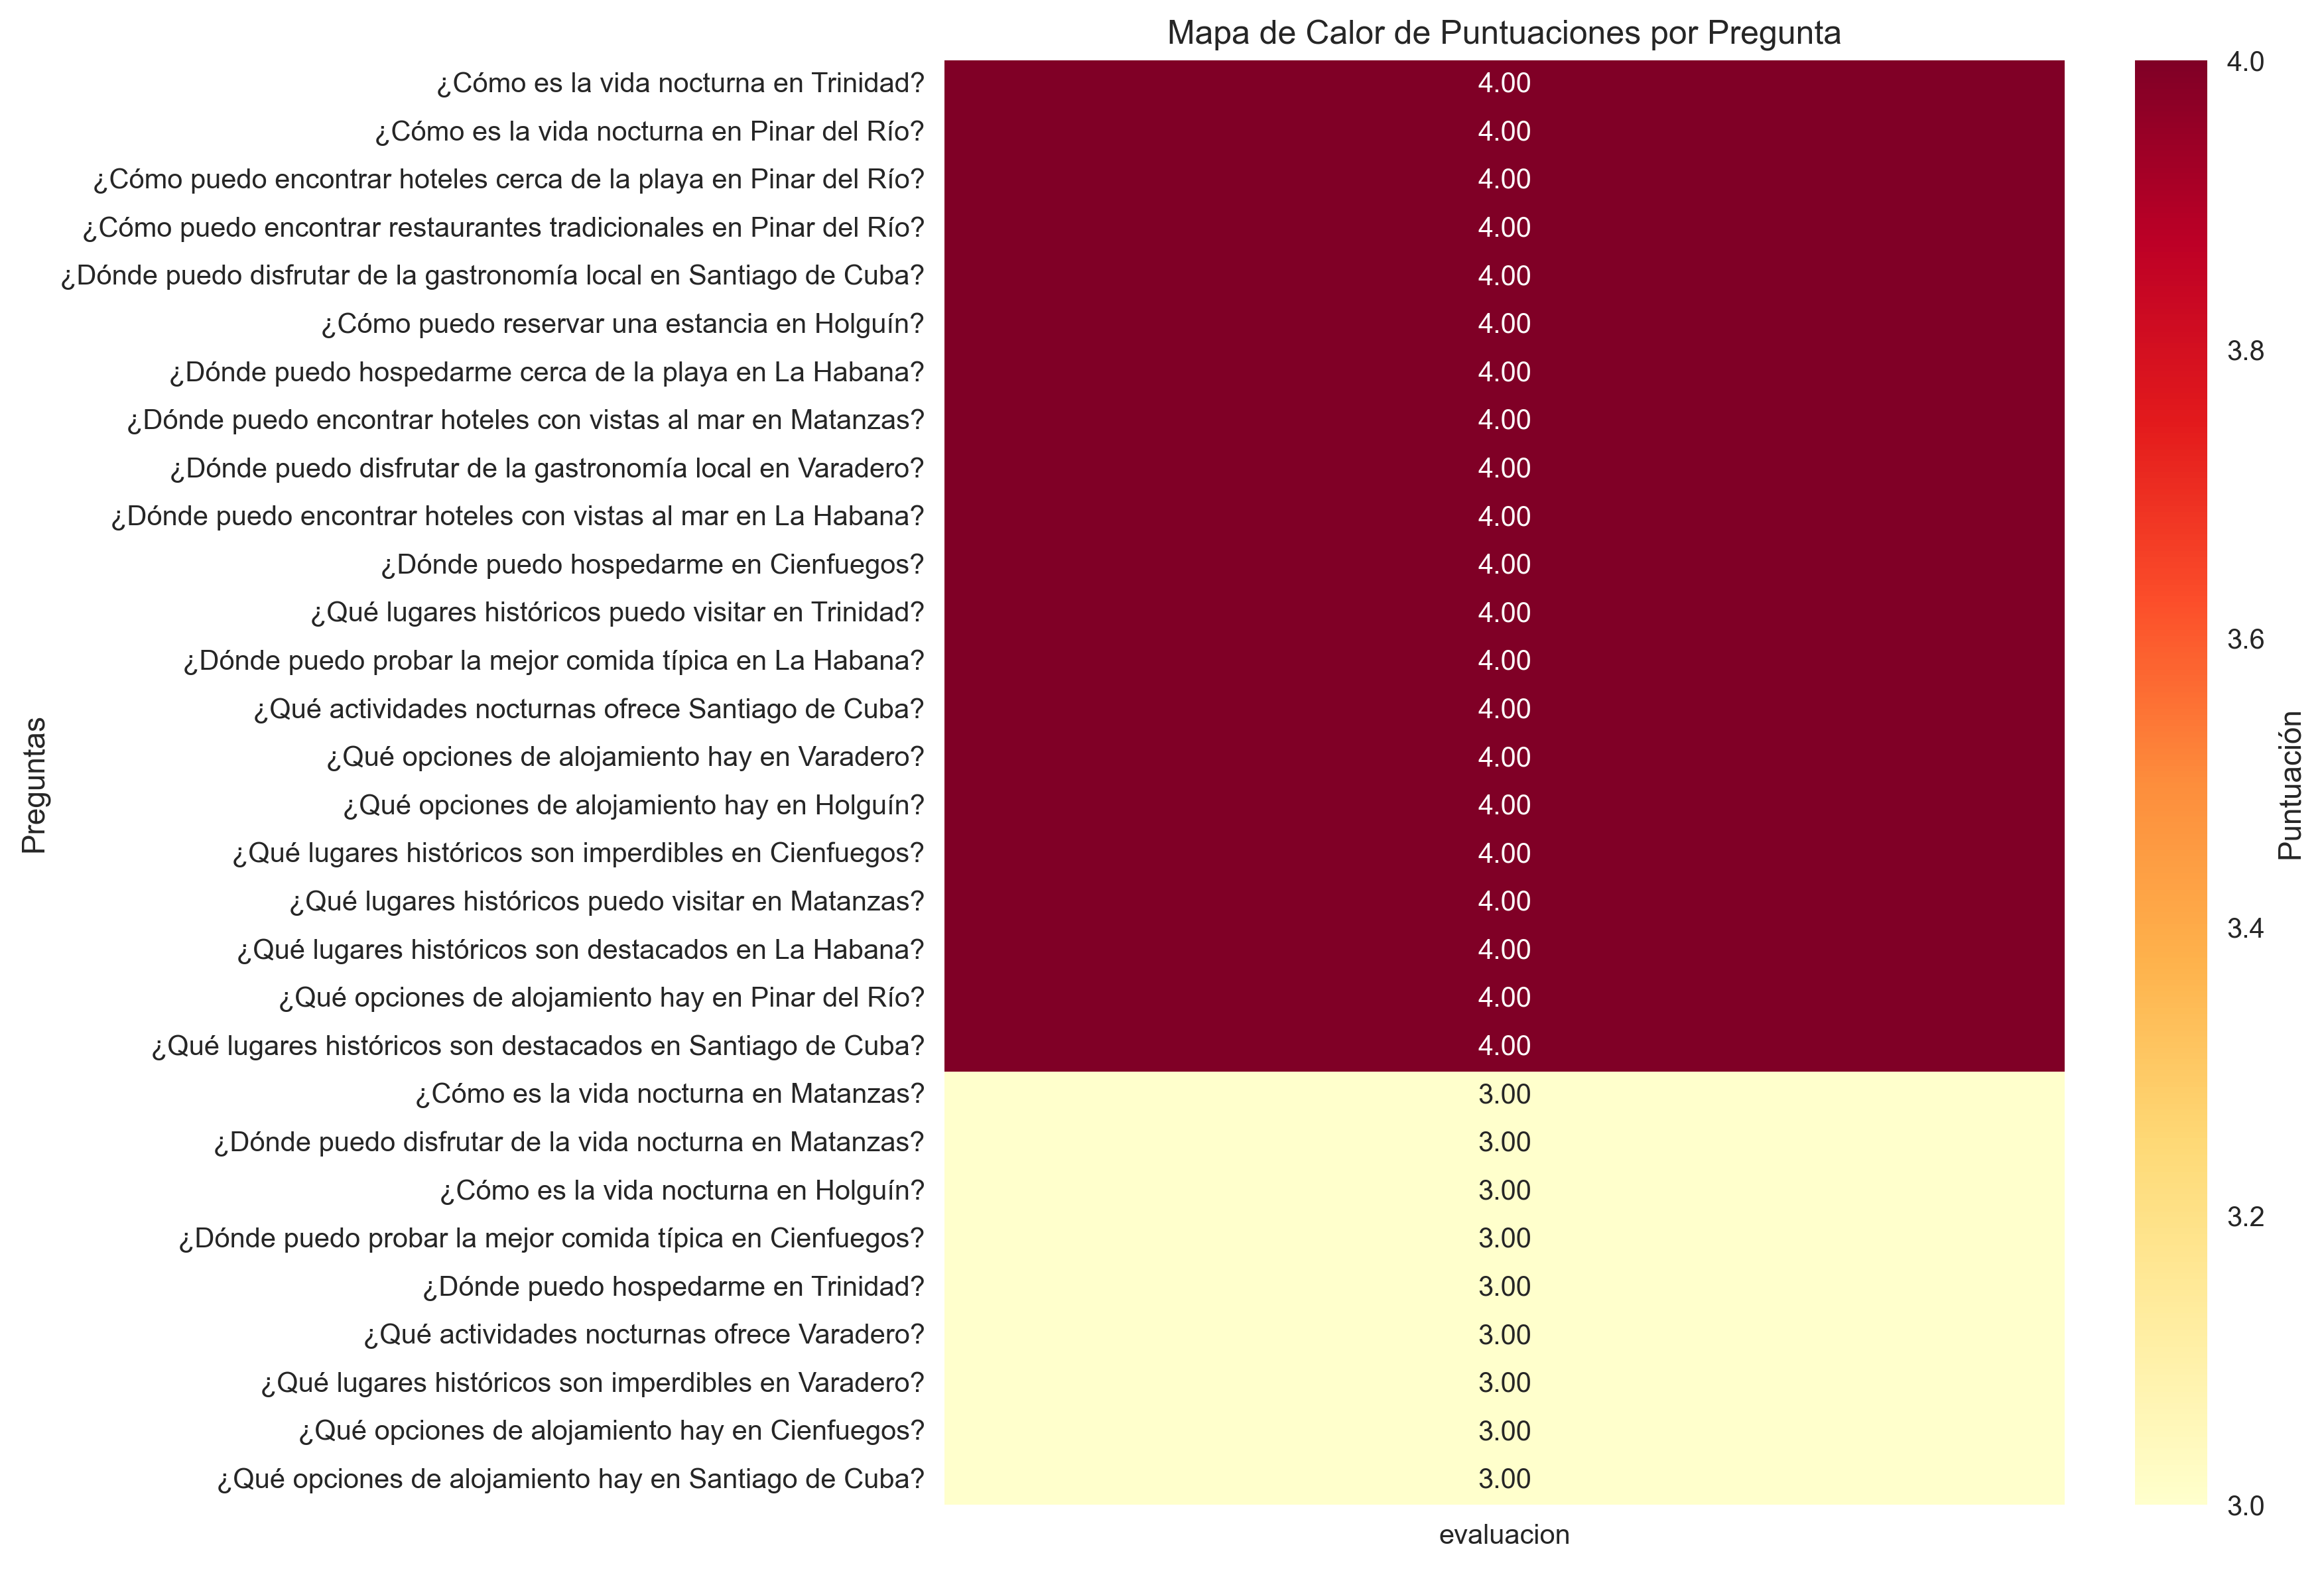
\includegraphics[width=1\textwidth]{../src/experiments/one_only_agent/quality_heatmap_20250614-143724.png}
\caption{Evaluaciones obtenidas para la respuesta a cada pregunta en la muestra más pequeña (tamaño 30)}
\label{fig:eval_1}
\end{figure}

\begin{remark}
Se obtuvo un intervalo de confianza de $[3.6499..., 3.75]$, lo que indica unos resultados aceptables. 
La Figura {\figref{fig:boot_dist_1}} muestra la distribución bootstrap de la puntuación media y la figura
{\figref{fig:eval_1}} muestra un mapa de calor con las puntuaciones otorgadas a las respuestas del sistema a las 
30 preguntas iniciales.
\end{remark}

\subsubsection{Sistema con Agentes Especializados }

La Tabla \tabref{tab:boot_results_2} resume las métricas clave obtenidas:

\begin{table}[h]
\centering
\caption{Resultados del análisis de bootstrapping (IC 95\%)}
\label{tab:boot_results_2}
\begin{tabular}{lccc}
\hline
\textbf{Métrica} & \textbf{Tamaño=30} & \textbf{Tamaño=300}  \\
\hline 
Puntuación Media& 4.1333... & 4.1329...  \\
Desviación Estándar & 0.6182... & 0.0349...  \\
\hline
\end{tabular}
\end{table}

\begin{figure}[h]
\centering
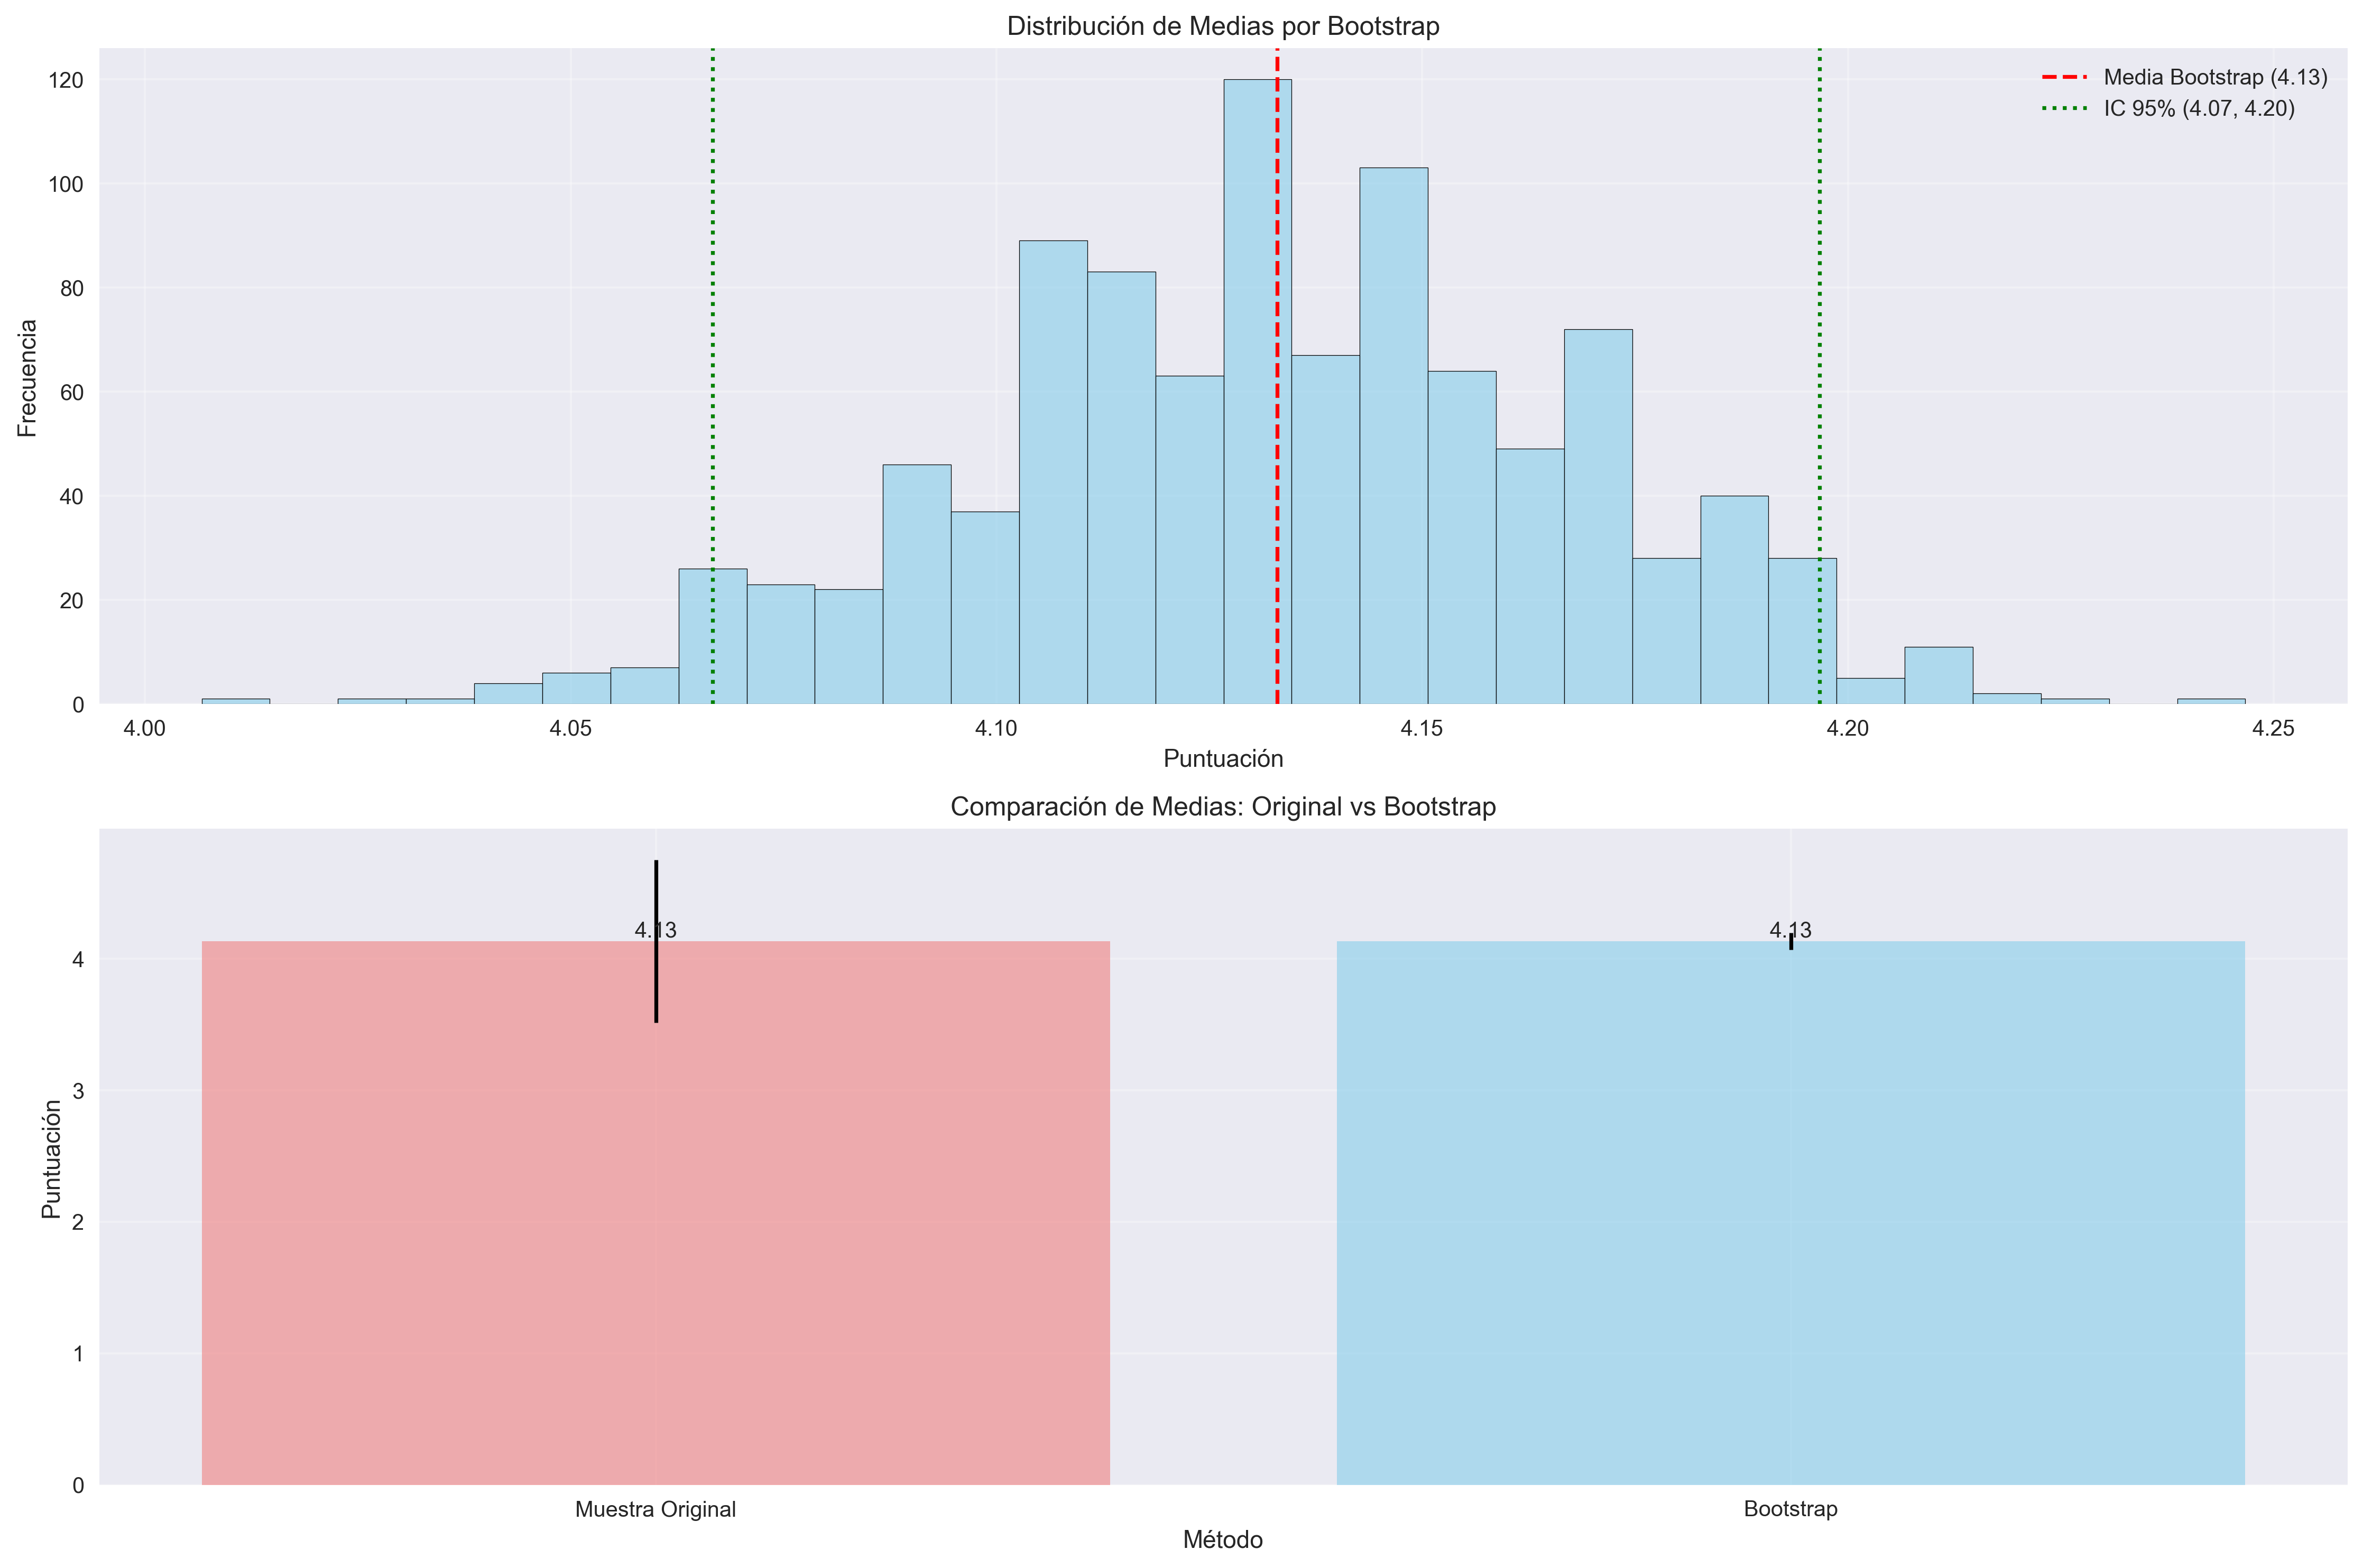
\includegraphics[width=1\textwidth]{../src/experiments/specialized_agents/bootstrap_distribution_20250614-005640.png}
\caption{Distribución bootstrap de la puntuación media ($N=1000$). La línea discontinua roja indica la media bootstrap (4.13)}
\label{fig:boot_dist_2}
\end{figure}

\begin{figure}[h]
\centering
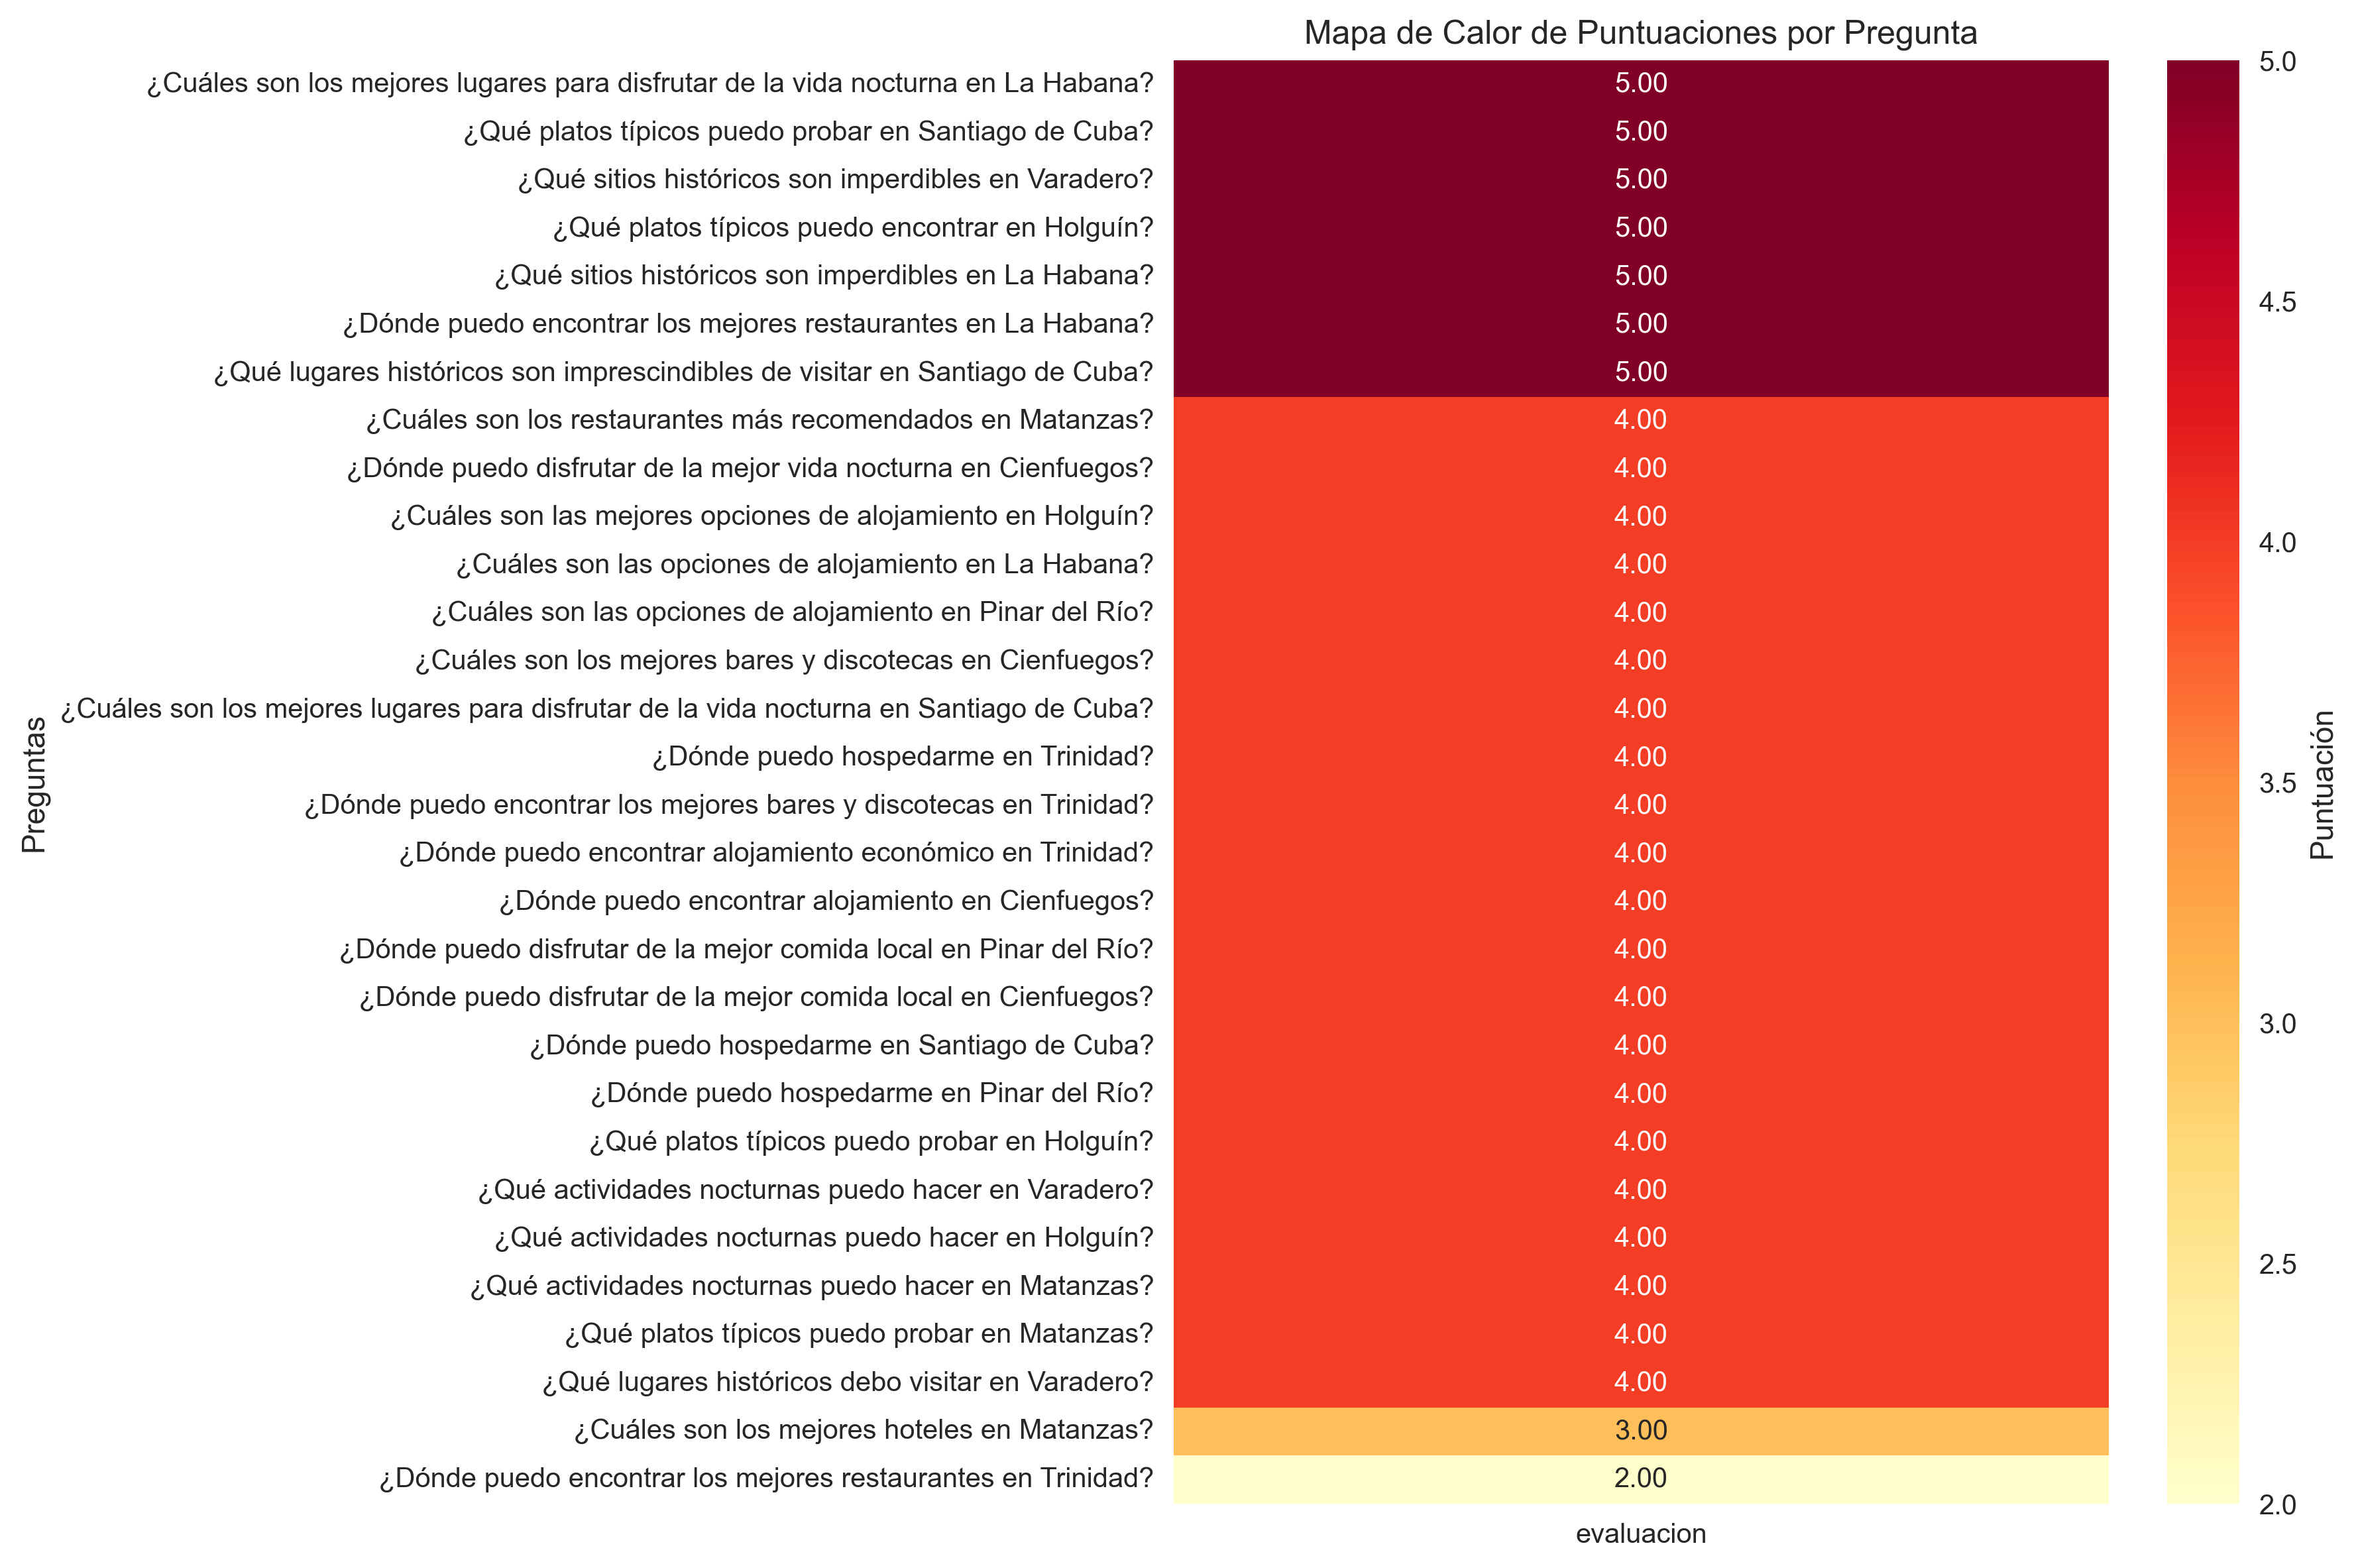
\includegraphics[width=1\textwidth]{../src/experiments/specialized_agents/quality_heatmap_20250614-005640.png}
\caption{Evaluaciones obtenidas para la respuesta a cada pregunta en la muestra más pequeña (tamaño 30)}
\label{fig:eval_2}
\end{figure}

\begin{remark}
Se obtuvo un intervalo de confianza de $[4.0666...,4.1966...]$, lo que indica unos resultados bastante buenos. 
La Figura {\figref{fig:boot_dist_2}} muestra la distribución bootstrap de la puntuación media y la figura 
{\figref{fig:eval_2}} muestra un mapa de calor con las puntuaciones otorgadas a las respuestas del sistema a las 
30 preguntas iniciales.
\end{remark}

En resumen, se puede observar que al añadir agentes especializados al sistema, mejoró la respuesta del modelo, lo cual demostró 
que la decisión tomada estuvo acertada.

\end{document}